\section{Collaboration networks: formation, bridges, and disciplinary exchange}
\label{sec:collaboration}

\subsection{Corpus and network construction}

The collaboration analysis was rebuilt from the same 29,139-record, 1972--2025 corpus used for the review's publication and topic results. Two records have no usable publication year. Among the dated records, two duplicate document identifiers were collapsed, leaving 29,135 unique dated records. Author lists were available for 29,016 of these. The remaining 119 records were retained in the review corpus but could not contribute author--author links. These counts distinguish the corpus denominator from the observable coauthorship denominator.

Author names were canonicalized with the same identity rules used in the earlier analysis, while preserving byline order for BAL author-position credit. An undirected edge joins two authors who appear on the same paper. Following the original network algorithm, a paper with $n$ authors adds $1/(n-1)$ to each of its coauthor edges; repeated joint papers accumulate weight. This reduces the influence of a single large team while preserving repeated collaboration. Core authors were selected by the original BAL measure, the mean rank of position-weighted fractional output and domain/year-normalized summed citations. The top 800 BAL authors were retained, isolated authors were removed, and the largest connected component was used for the community map. Weighted Louvain detection used the original deterministic partition routine and resolution 1.0. The temporal analysis uses the full observable author network, rather than only this selected core.

The complete coauthorship graph contains 70,603 authors with at least one coauthor and 271,869 distinct pairs. Its largest connected component contains 42,425 authors, or 60.1\% of coauthor nodes. Among the BAL top 800, 630 remain after isolates are removed; their largest component has 554 authors and 1,446 links. Weighted Louvain yields 36 communities with modularity $Q=0.8924$. These values replace the previous estimates obtained from the smaller 23,280-paper network. Figure~\ref{fig:collab_communities} shows the rebuilt core with every author named. A companion SVG vector figure supports zooming to read individual names.

\begin{figure}[htbp]
\centering
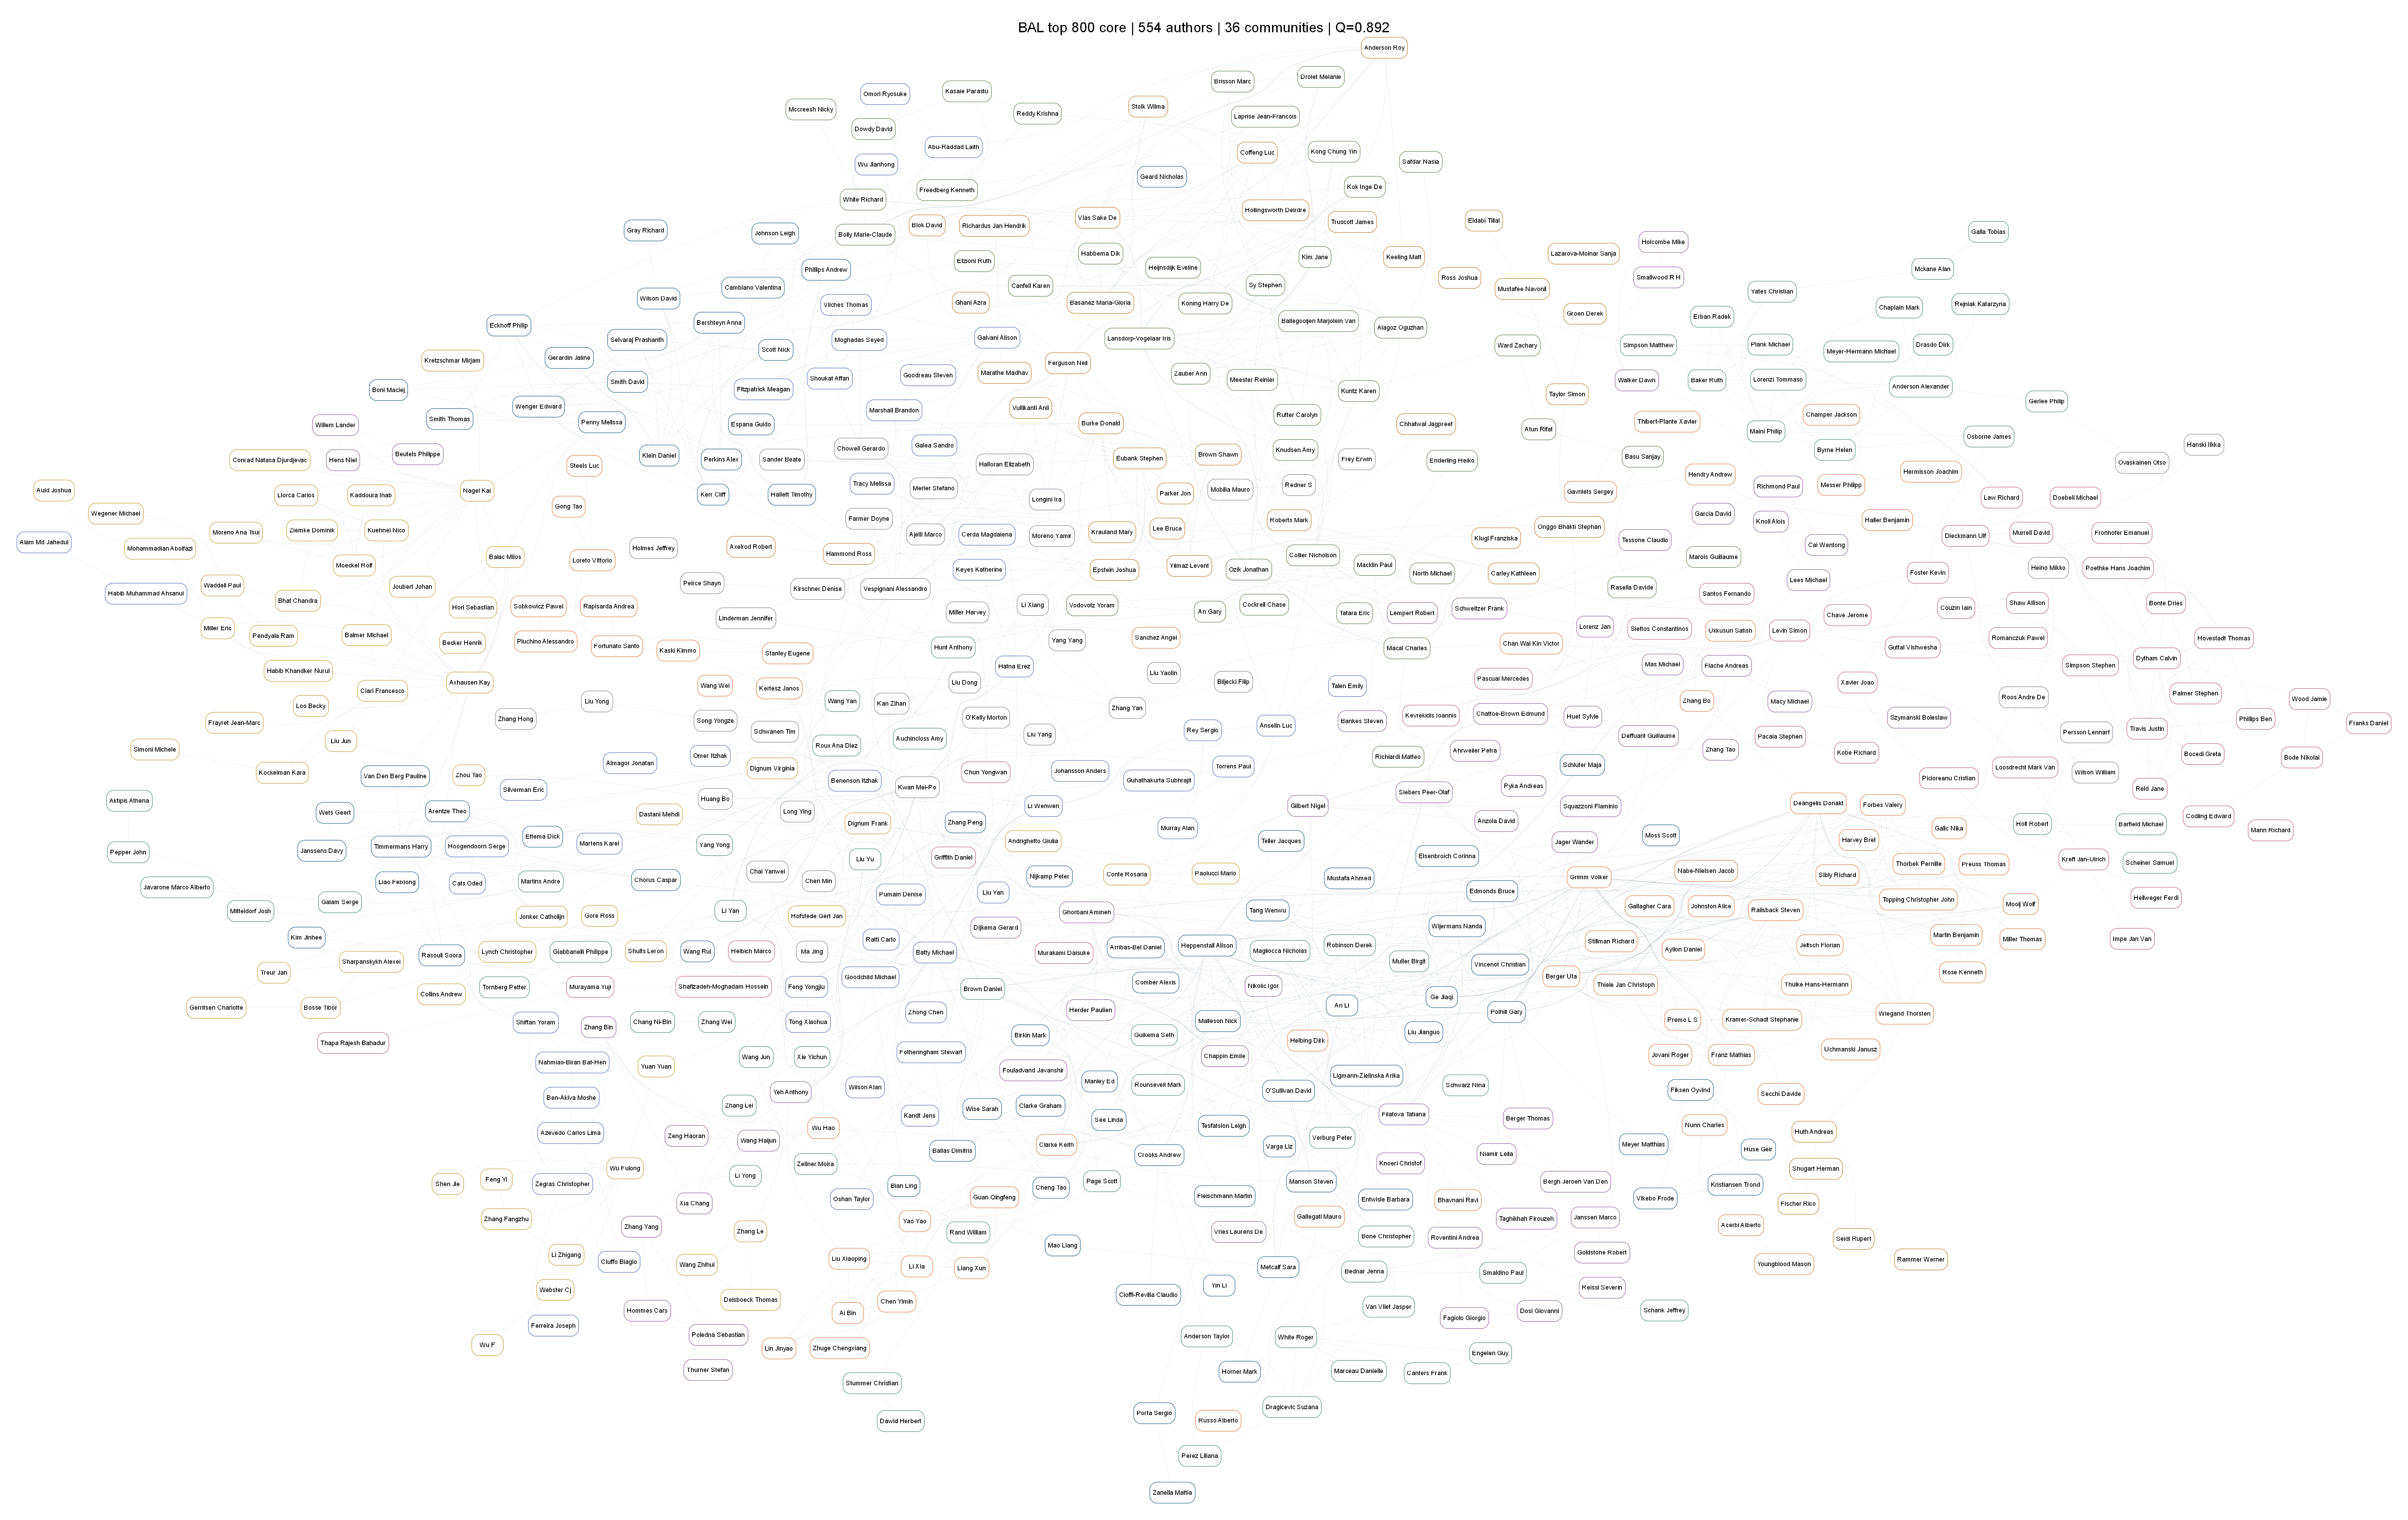
\includegraphics[width=0.94\textwidth,height=0.75\textheight,keepaspectratio]{figures/collab_29139_author_communities.png}
\setcounter{figure}{13}
\caption{Fully labelled author collaboration core from the 29,139-record corpus. Every one of the 554 authors in the largest connected component of the BAL top 800 is named. Box outline color indicates weighted Louvain community, and lines indicate coauthorship. The separate SVG version is intended for close reading at full resolution.}
\label{fig:collab_communities}
\end{figure}

\subsection{Formation and persistence of collaboration}

To distinguish expansion from continuity, we counted a distinct author pair once within each time period. A \emph{new pair} had not appeared in any earlier period; a \emph{repeated pair} had appeared previously. Consecutive-period survival is the fraction of pairs in the preceding period that reappear in the next. The periods retain the earlier manuscript's breakpoints. Because the intervals have unequal lengths, new-pair counts are also shown per year and survival rates should be read as descriptive period summaries rather than standardized hazards.

\begin{table}[htbp]
\centering
\small
\setlength{\tabcolsep}{5pt}
\caption{Formation and persistence of coauthorship ties in the observable network}
\label{tab:collab_temporal}
\begin{tabular}{lrrrrrr}
\toprule
Period & Papers & Authors & New pairs & Repeated pairs & Prior ties surviving & Largest component \\
 & & & per year & (\% of current) & (\%) & (\% of authors) \\
\midrule
1972--2005 & 1,862 & 3,594 & 181 & 0.0 & --- & 5.2 \\
2006--2012 & 4,577 & 10,377 & 3,276 & 1.2 & 4.5 & 12.3 \\
2013--2015 & 3,603 & 9,941 & 7,577 & 6.0 & 6.1 & 10.9 \\
2016--2025 & 18,974 & 54,576 & 22,006 & 1.6 & 12.1 & 54.7 \\
\bottomrule
\end{tabular}
\end{table}

\begin{figure}[htbp]
\centering
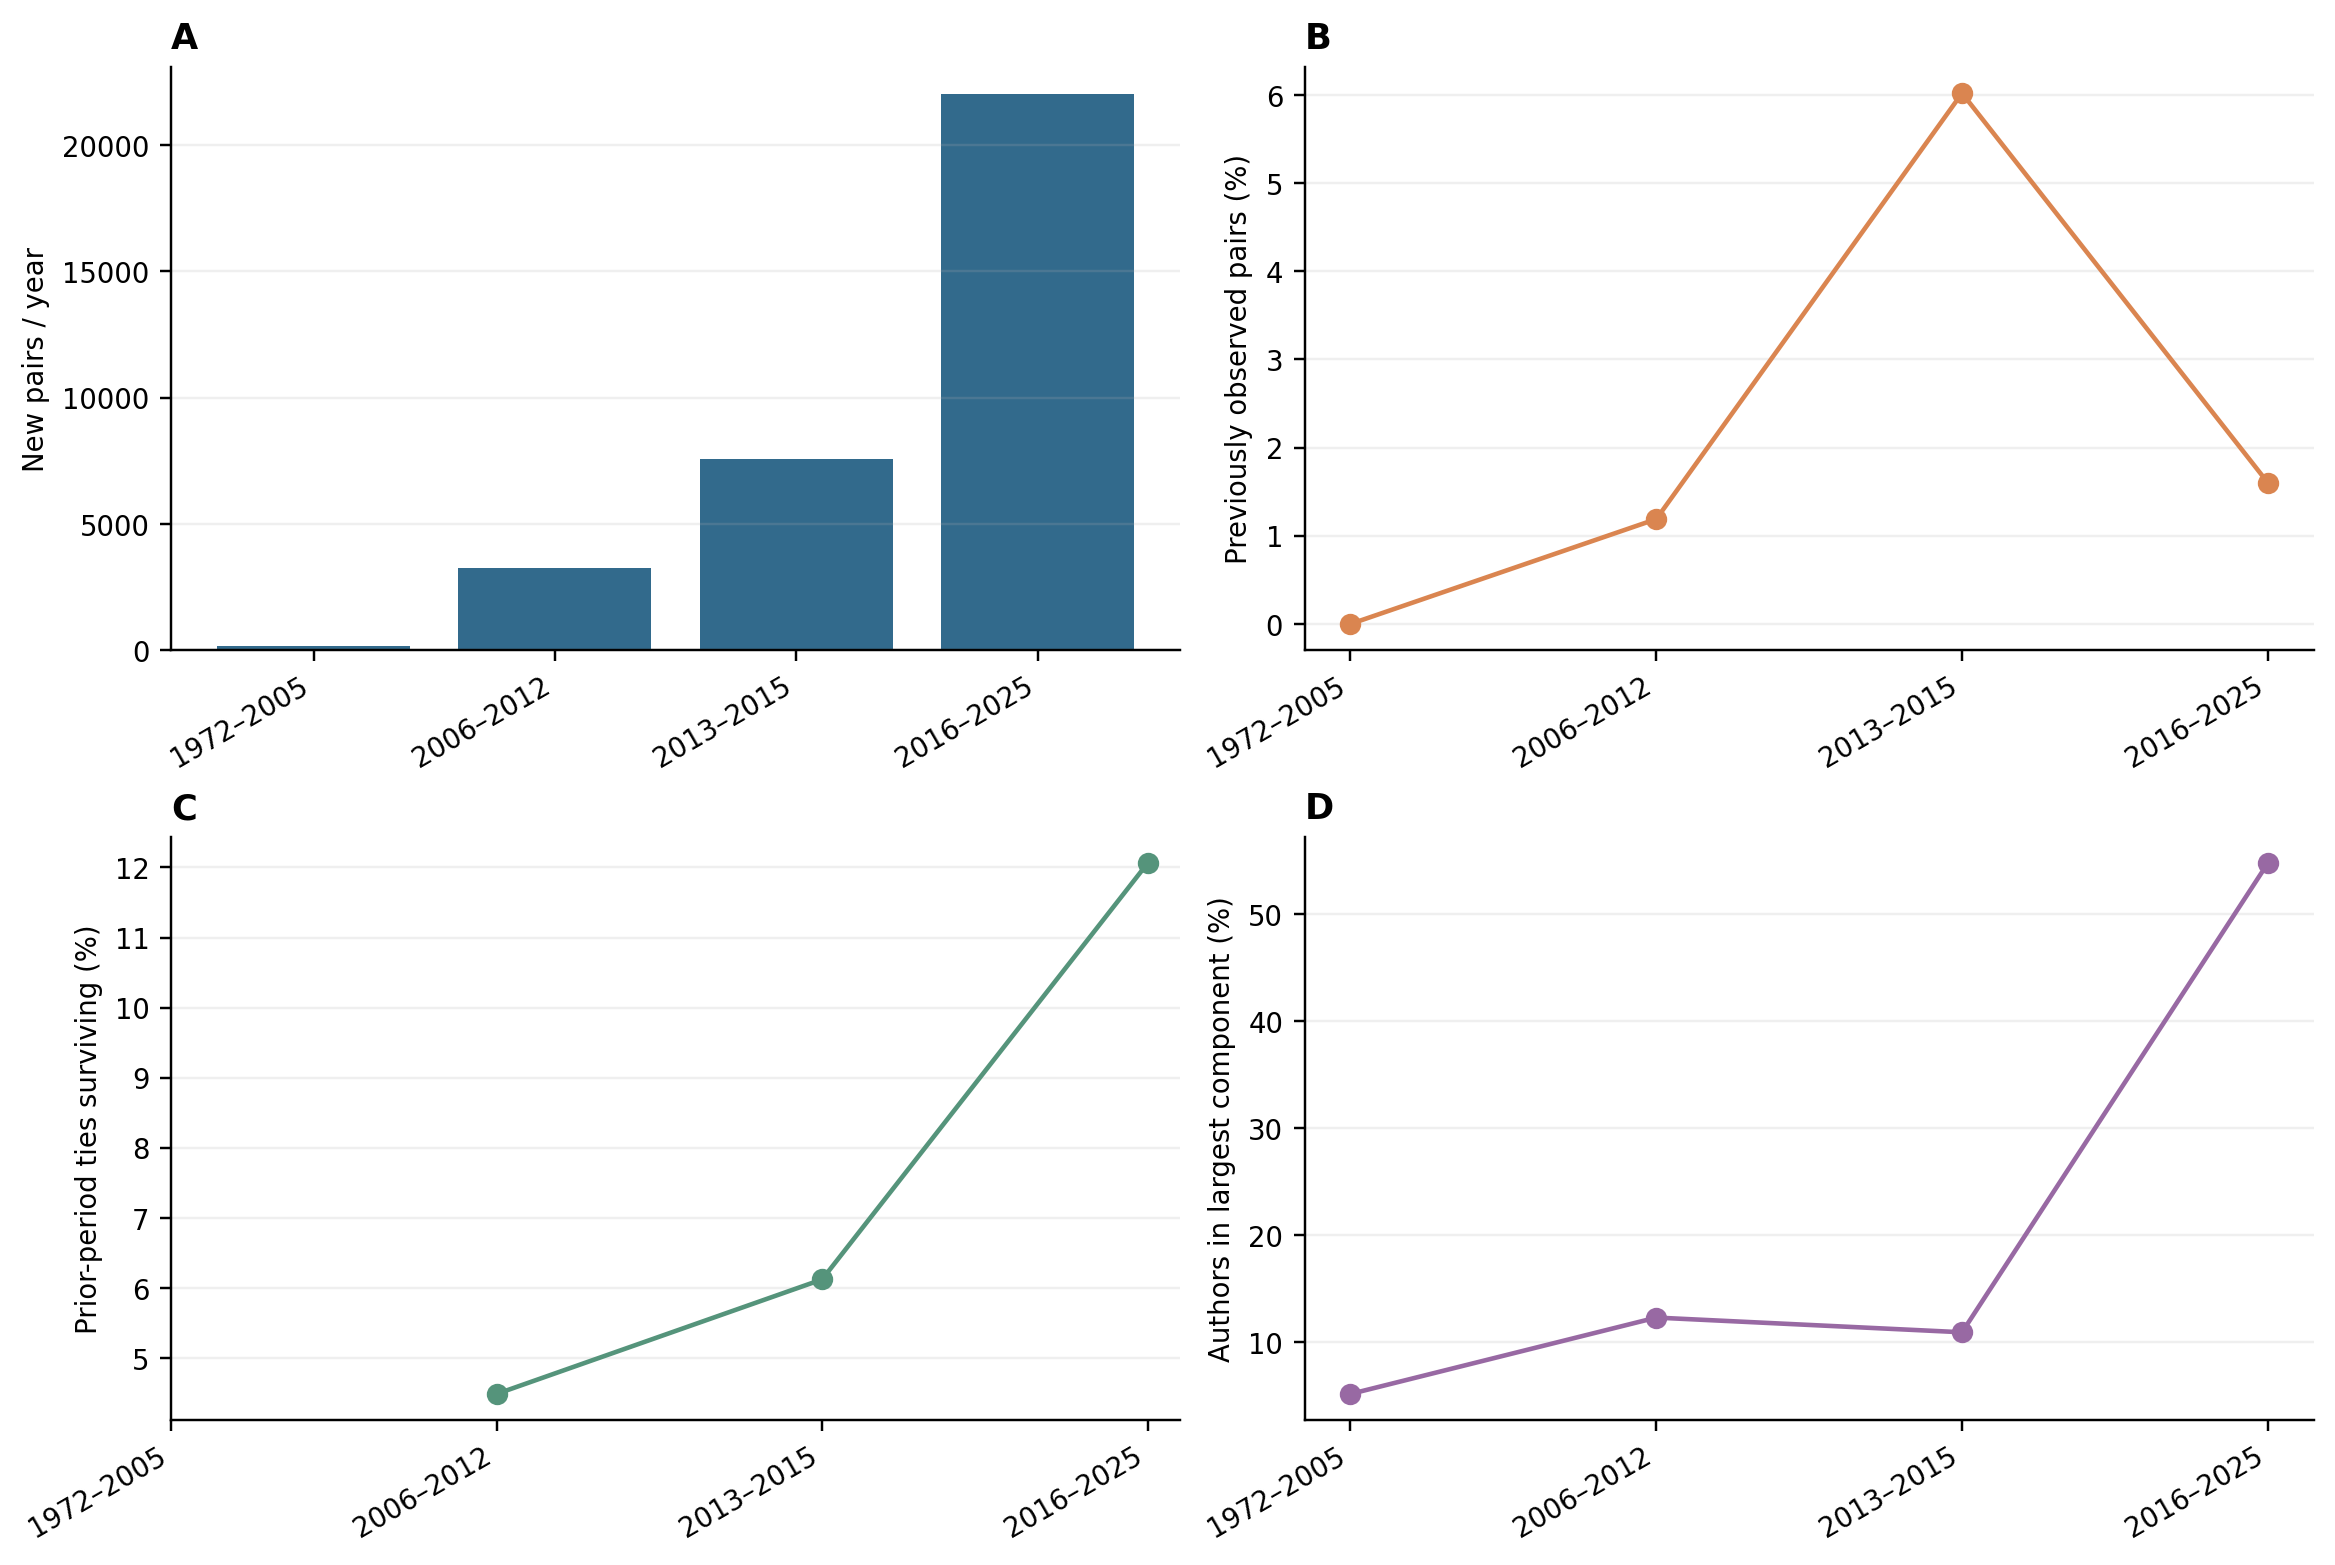
\includegraphics[width=0.96\textwidth,height=0.78\textheight,keepaspectratio]{figures/collab_29139_temporal_ties.png}
\caption{New and repeated coauthor pairs, adjacent-period tie survival, and the largest-component share. The periods follow the previous analysis and have different durations.}
\label{fig:collab_temporal}
\end{figure}

New collaborations accelerated sharply: 6,149 distinct pairs first appeared by 2005, compared with 22,934 in 2006--2012, 22,731 in 2013--2015, and 220,055 in 2016--2025. The annualized figures in Table~\ref{tab:collab_temporal} account for the different period lengths. Yet most links in every later interval were newly observed. Only 1.6\% of pairs active in 2016--2025 had been seen in an earlier period. This low repeated-pair share partly reflects the influx of new authors and should not be interpreted as evidence that established teams ceased collaborating. Of pairs present in 2013--2015, 12.1\% recur in 2016--2025, higher than the preceding adjacent-period overlap. The later interval is longer, which also increases the opportunity to observe a recurrence.

The largest-component share rose from 5.2\% in the first period to 54.7\% in 2016--2025. This indicates that more authors became connected through chains of coauthorship, even though the directly repeated ties remained a small fraction of the rapidly growing edge set. The temporary decrease from 12.3\% in 2006--2012 to 10.9\% in 2013--2015 cautions against describing the trajectory as uniformly monotonic. Figure~\ref{fig:collab_temporal} separates these four aspects of growth.

\subsection{Community boundaries and bridge authors}

High modularity describes a field organized around comparatively dense local collaboration. It does not mean the groups are completely isolated. In the 554-author core, 355 of 1,446 links (24.6\%) cross a Louvain community boundary, but these links carry only 6.2\% of total collaboration weight. Cross-community contacts therefore tend to involve fewer repeated joint papers than within-community contacts. An unweighted Louvain run on the same core still finds 36 communities, with $Q=0.6971$; the difference in modularity shows that repeated collaboration strengthens the observed boundaries.

Two measures identify different roles in connecting this structure. Betweenness centrality counts how often an author lies on shortest paths between other authors. The participation coefficient, $P_i=1-\sum_c(s_{ic}/s_i)^2$, measures how evenly the author's weighted ties are distributed across communities. Michael Batty has high betweenness (0.119) and participation (0.566), consistent with a bridge role in this selected graph. Bruce Edmonds (0.053; 0.663), Peer-Olaf Siebers (0.057; 0.632), Virginia Dignum (0.069; 0.588), and Amineh Ghorbani (0.103; 0.462) also combine path brokerage with diverse community ties. In contrast, Volker Grimm has even higher betweenness (0.207) but lower participation (0.294), and Kay Axhausen has participation of 0.121. Their importance to paths through the graph is therefore distinct from how broadly their direct collaboration is distributed across communities. These are positions within the BAL-selected coauthorship graph, not measures of individual scientific merit.

\begin{figure}[htbp]
\centering
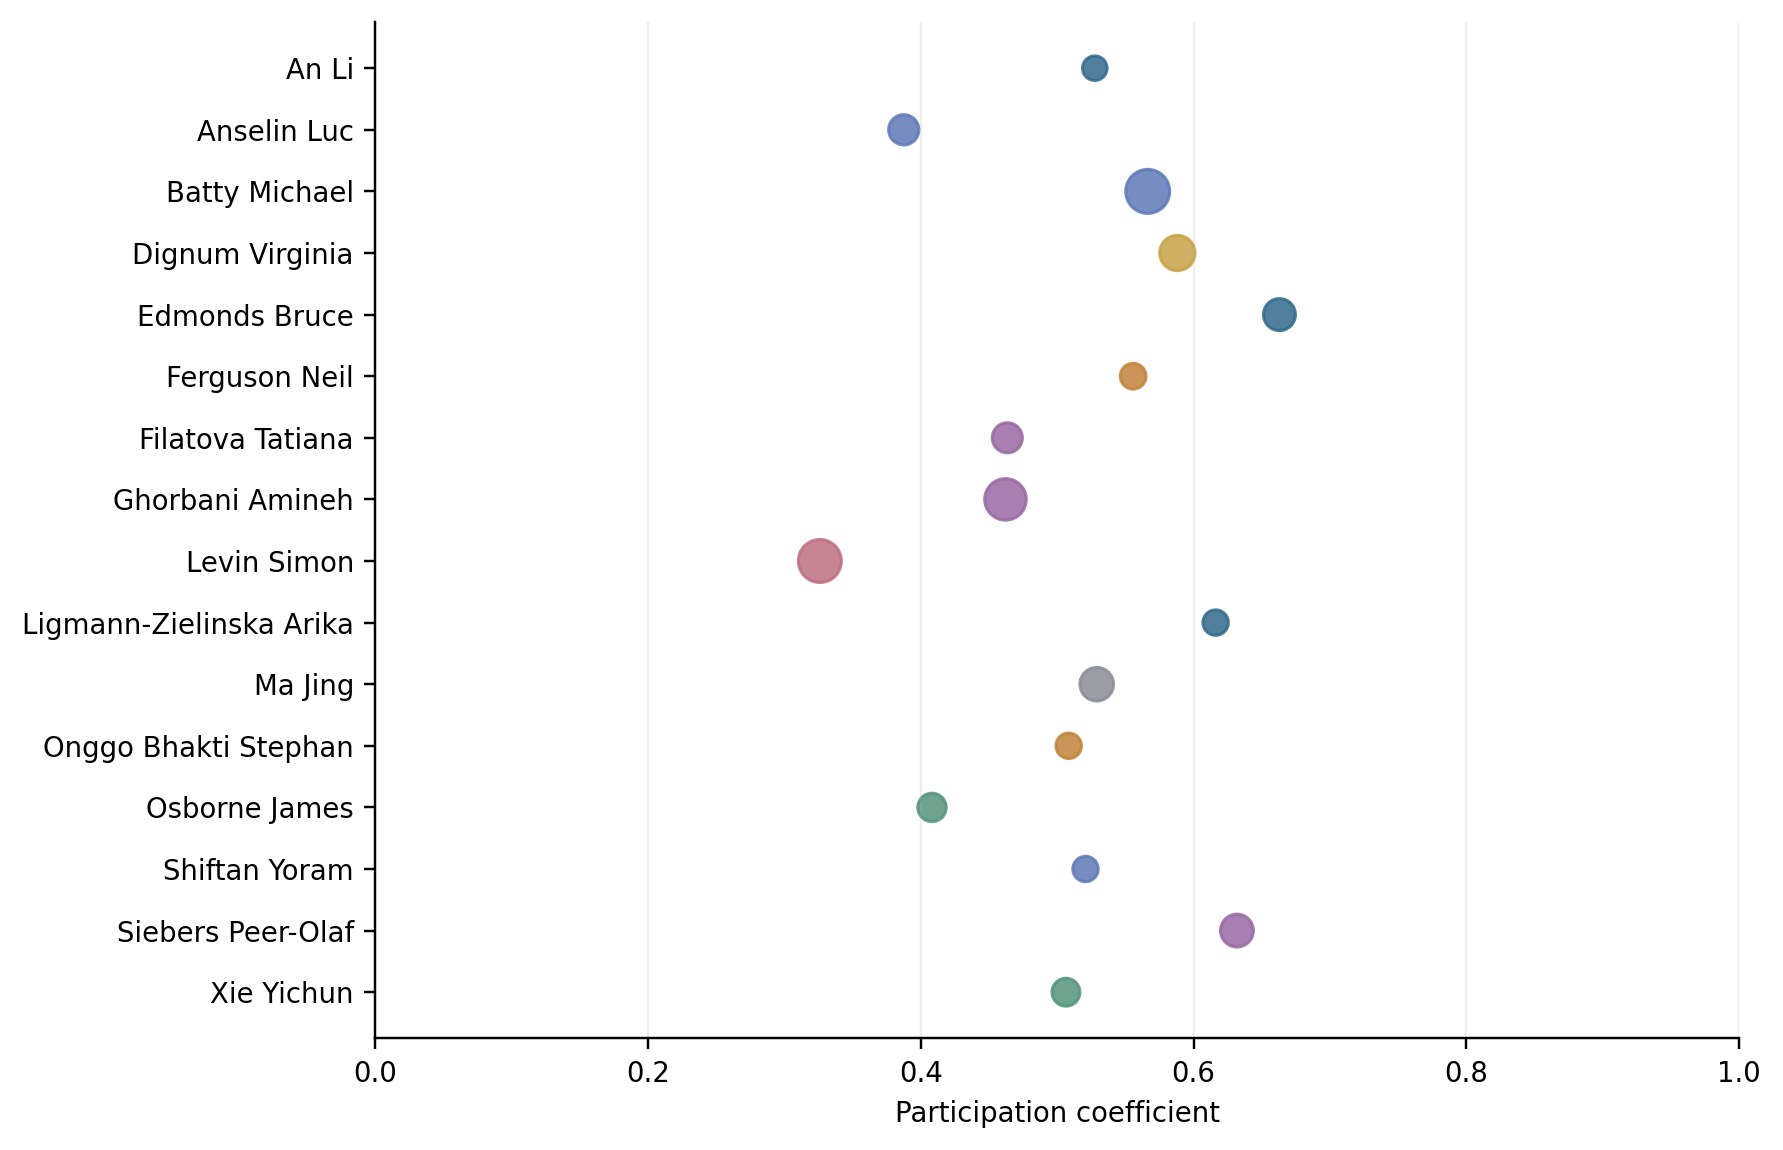
\includegraphics[width=0.90\textwidth,height=0.75\textheight,keepaspectratio]{figures/collab_29139_bridge_authors.png}
\caption{Authors combining high path betweenness and participation across communities. Bubble area reflects betweenness; horizontal position gives the participation coefficient.}
\label{fig:collab_bridges}
\end{figure}

\subsection{Cross-domain collaboration}

We linked each detected community to the primary topics of papers authored by its members. Some communities have clear concentrations: environmental research accounts for 75.8\% of papers associated with community C2, public health for 89.3\% of C8, and transport for 66.1\% of C5. Others are heterogeneous. The leading topic in C1 accounts for only 22.3\%, and that in C3 for 28.6\%; these groups should not be assigned a single disciplinary identity. For descriptive community-to-community comparisons, we labelled a group by its modal topic only when that topic covered at least 35\% of its associated papers.

To test whether collaboration itself spans fields, we also assigned each author a primary domain from the plurality of their papers in the observable corpus. Among multi-author papers for which at least two authors could be assigned domains, the share combining authors from different home domains was 18.5\% in 1972--2005, 25.9\% in 2006--2012, 28.4\% in 2013--2015, and 27.4\% in 2016--2025. Thus cross-domain teamwork became more common than in the early period, but the last two periods do not support a continued increase. The author-domain assignment uses the full observation window, so these percentages describe the final corpus retrospectively rather than measuring a time-varying disciplinary identity.

Public health--environment is the largest cross-domain pair in absolute paper-equivalent volume (1,508), followed by public health--social dynamics (634) and public health--transport (534). Transport--urban/land use contributes 363. Energy--urban/land use (16) and energy--swarm/robotics (14) have much smaller observed volumes. These are counts, not opportunity-adjusted collaboration propensities: small fields can have low pair volumes even if their members are relatively willing to collaborate. Figure~\ref{fig:collab_domains} displays both the time trend and the domain-pair matrix.

\begin{figure}[htbp]
\centering
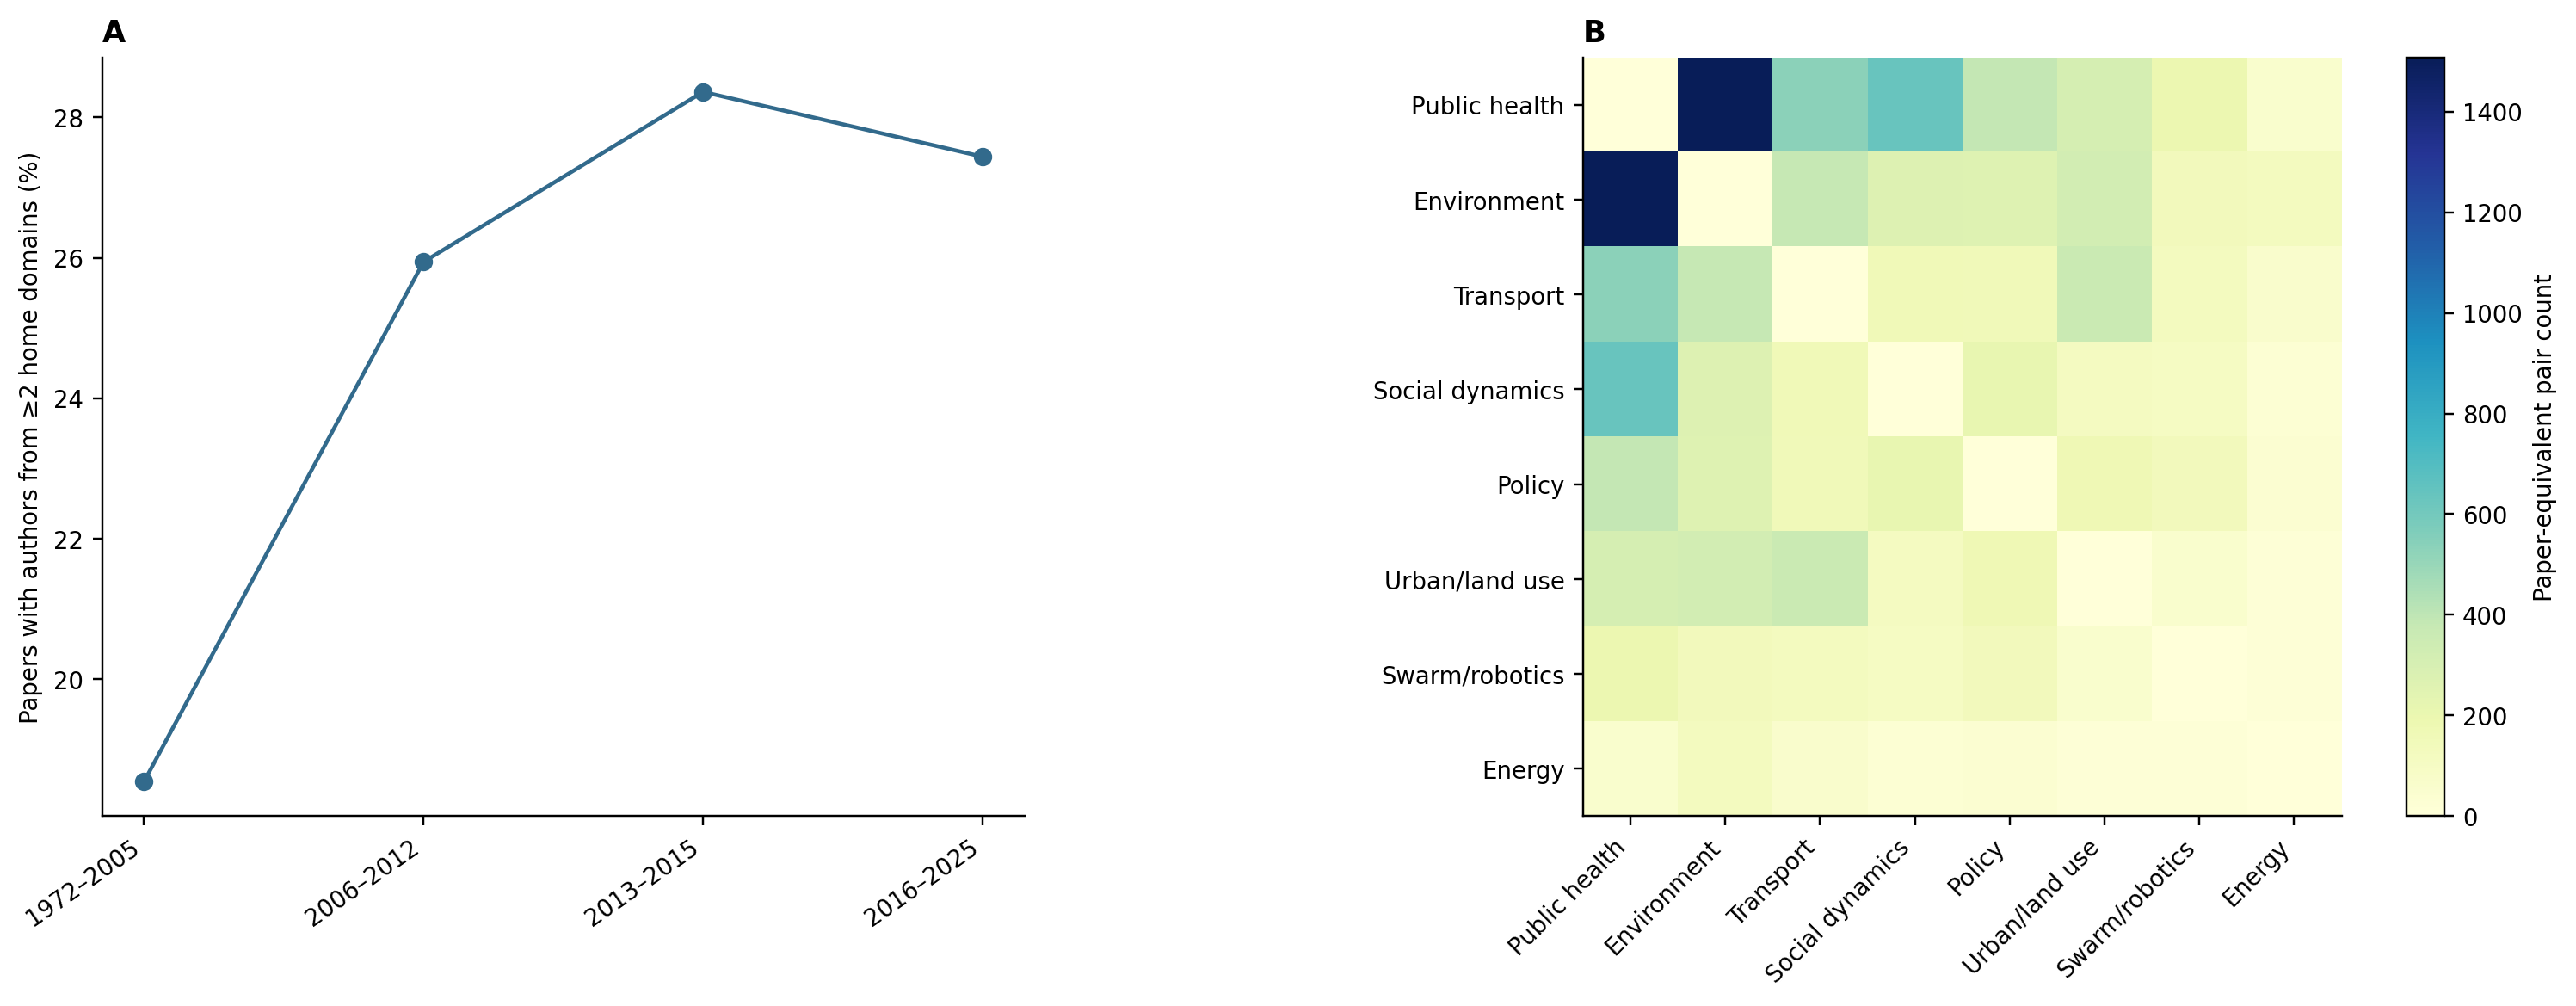
\includegraphics[width=0.98\textwidth,height=0.70\textheight,keepaspectratio]{figures/collab_29139_cross_domain.png}
\caption{Cross-domain coauthorship in the 29,139-record corpus. Panel A shows the share of eligible papers whose coauthors have at least two different primary domains. Panel B shows paper-equivalent coauthor-pair volume across domains; each cross-domain paper contributes total weight one across its different-domain author pairs.}
\label{fig:collab_domains}
\end{figure}

\subsection{Interpretation and limitations}

The expanded corpus portrays a connected but internally structured research field. Large-scale growth has made a majority of coauthor nodes reachable through the largest component, while recurrent collaboration remains concentrated within communities. A subset of authors connects these groups, and the most visible cross-domain paths involve public health, environment, and transport. The distinction between edge presence, repeated edge weight, shortest-path position, and topical mixing is essential: each captures a different form of integration.

The analysis inherits several limits of bibliographic coauthorship data. Canonical name strings can merge distinct people or split one person, author-order credit conventions do not apply equally across fields, and missing author metadata removes 119 unique dated records from network construction. BAL selection is designed to make a readable core and does not represent all 70,603 coauthor nodes. Community labels and modularity depend on this selection and on edge weighting. Finally, a coauthored paper documents a collaboration but does not reveal the direction of knowledge transfer or the quality of intellectual exchange. The figures should therefore be read as a reproducible map of observed collaboration, not as a complete account of disciplinary integration.
